% \input{"IAB/latex/TeX-Folienformat.tex"}
\input{"/Users/jonathanlatner/Google Drive/My Drive/IAB/latex/TeX-Folienformat.tex"}

\documentclass[t,8pt,utfx8]{beamer}
\usepackage{booktabs}
\usepackage{setspace}
\usepackage{parskip}
\usepackage{graphicx}
\usepackage{subcaption}
\setbeamertemplate{caption}[numbered]
\newcommand{\sprache}{\englisch}
\renewcommand{\thesubsection}{\alph{subsection})}
\usepackage[cal=pxtx, scr=dutchcal]{mathalpha}


\newcommand{\btVFill}{\vskip0pt plus 1filll}

\title[Its complicated: Know your data and know your generator. Comparing efficiency, utility, and privacy between synthetic data packages and methods]{Its complicated: Know your data and know your generator}
\subtitle{Wiesbaden, \newline 21. März, 2024}

\author{Jonathan Latner, PhD \newline Dr. Marcel Neuenhoeffer \newline Prof. Dr. Jörg Drechsler}

\newcounter{noauthorlines}
\setcounter{noauthorlines}{2} % Wert für 2 Autoren über 2 Zeilen. Ggf. anpassen

% %%%%%%%%%%%%%%
% Ende Anpassung
% %%%%%%%%%%%%%%

% \input{"IAB/latex/TeX-Folienformatierung_CD_2019"}
\input{"/Users/jonathanlatner/Google Drive/My Drive/IAB/latex/TeX-Folienformatierung_CD_2019"}

% Modify the section in toc template to enumerate
\setbeamertemplate{section in toc}{%
    \inserttocsectionnumber.~\inserttocsection\par
}

% use for subsections
% \setbeamertemplate{subsection in toc}{}
\setbeamertemplate{subsection in toc}{%
    \setlength{\parskip}{1mm}
        \hskip2mm -- \hskip1mm\inserttocsubsection\par
}


\usepackage{colortbl}
\definecolor{lightgray}{gray}{0.9}


\begin{document}


\frame[plain]{\titlepage}

\begin{spacing}{1.25}

%Table of contents
\begin{frame}
\frametitle{Sections}
\vskip6mm
\setlength{\leftskip}{0.5mm}
\setlength{\parskip}{5mm}
\begin{NoHyper}
    \tableofcontents
\end{NoHyper}
\end{frame}

\section{Introduction}\label{sec:intro}
\frame[c]{\frametitle{}
\centering
Section \ref{sec:intro}: Introduction
}

\frame{\frametitle{Compare 3 Synthetic Data Generator (SDG)}
\begin{itemize}
    \item DataSynthesizer (Bayes)
    \item CTGAN (GAN)
    \item Synthpop (CART)
\end{itemize}
}


\section{Know your data (SD2011)}\label{sec:data}
\frame[c]{\frametitle{}
\centering
Section \ref{sec:data}: Know your data (SD2011)
}

\frame{\frametitle{Real data}
\begin{itemize}
    \item Social Diagnosis 2011 (SD2011)
    \item Loads with Synthpop
    \begin{itemize}
        \item \url{http://www.diagnoza.com/index-en.html}
        \item Not entirely clear how original data is created or cleaned to create data in Synthpop
    \end{itemize}
    \item Like real data, has `quirks' or unusual values/variables
    \begin{itemize}
        \item Includes missings
        \begin{itemize}
            \item Informative (i.e. month married, but single)
            \item Non-informative 
        \end{itemize}
        \item Includes `errors'
        \begin{itemize}
            \item \texttt{smoke} - Does not smoke is NO, but \texttt{nociga} - 20/22 cigarettes per day 
        \end{itemize}
        \item Includes generated variables
        \begin{itemize}
            \item \texttt{bmi,agegr}
            \item Can be problematic for SDG 
        \end{itemize}
    \end{itemize}
\end{itemize}
}


\frame{\frametitle{Data (SD2011)}
\vskip -5mm
\begin{table}[ht]
    \centering
    \vskip -2mm
    \rowcolors{1}{white}{lightgray}
    \resizebox{\textwidth}{!}{% latex table generated in R 4.4.0 by xtable 1.8-4 package
% Thu Sep 26 09:11:53 2024
\begin{tabular}{rlllllllll}
  \toprule
Number & Variable & Description & Type & Observations & Unique.Values & Missings & Negative.values & Generated & Messy \\ 
  \midrule
  1 & sex & Sex & factor & 5000 & 2 & 0 & 0 &  &  \\ 
    2 & age & Age of person, 2011 & numeric & 5000 & 79 & 0 & 0 &  &  \\ 
    3 & agegr & Age group, 2011 & factor & 5000 & 7 & 4 & 0 & Yes & Yes \\ 
    4 & placesize & Category of the place of residence & factor & 5000 & 6 & 0 & 0 &  &  \\ 
    5 & region & Region (voivodeship) & factor & 5000 & 16 & 0 & 0 &  &  \\ 
    6 & edu & Highest educational qualification, 2011 & factor & 5000 & 5 & 7 & 0 &  &  \\ 
    7 & eduspec & Discipline of completed qualification & factor & 5000 & 28 & 20 & 0 &  &  \\ 
   &  &  &  & \dots &  &  &  &  &  \\ 
   10 & income & Personal monthly net income & numeric & 5000 & 407 & 683 & 603 &  & Yes \\ 
   11 & marital & Marital status & factor & 5000 & 7 & 9 & 0 &  &  \\ 
   12 & mmarr & Month of marriage & numeric & 5000 & 13 & 1350 & 0 &  &  \\ 
   14 & msepdiv & Month of separation/divorce & numeric & 5000 & 13 & 4300 & 0 &  &  \\ 
   15 & ysepdiv & Year of separation/divorce & numeric & 5000 & 51 & 4275 & 0 &  &  \\ 
   &  &  &  & \dots &  &  &  &  &  \\ 
   22 & nofriend & Number of friends & numeric & 5000 & 44 & 0 & 41 &  & Yes \\ 
   23 & smoke & Smoking cigarettes & factor & 5000 & 3 & 10 & 0 &  &  \\ 
   24 & nociga & Number of cigarettes smoked per day & numeric & 5000 & 30 & 0 & 3737 &  & Yes \\ 
   &  &  &  & \dots &  &  &  &  &  \\ 
   28 & wkabdur & Total time spent on working abroad & numeric & 5000 & 33 & 0 & 4875 &  & Yes \\ 
   &  &  &  & \dots &  &  &  &  &  \\ 
   33 & height & Height of person & numeric & 5000 & 65 & 35 & 0 &  &  \\ 
   34 & weight & Weight of person & numeric & 5000 & 91 & 53 & 0 &  &  \\ 
   35 & bmi & Body mass index (weight - kg/(height - cm$^2$)*10000) & numeric & 5000 & 1396 & 59 & 0 & Yes & Yes \\ 
   \bottomrule
\end{tabular}
}
    \label{table:sd2011_data_structure}
\end{table}
}

\section{Know your generator}\label{sec:sdg}
\subsection{DataSynthesizer}\label{sec:sdg_datasynthesizer}
\frame[c]{\frametitle{}
\centering
Section \ref{sec:sdg}\ref{sec:sdg_datasynthesizer}: Know your generator (DataSynthesizer)
}

\frame{\frametitle{Tasks}
\begin{itemize} 
    \item Run default model - correlated attribute mode
    \item Hyperparameters
    \begin{itemize}
        \item $\epsilon$ DP: 0 (default 0.1)
        \item Bayesian network ($\mathcal{N}$) parents: 1, 2, or 3 (default is `greedy')
    \end{itemize}
\end{itemize}
\begin{figure}
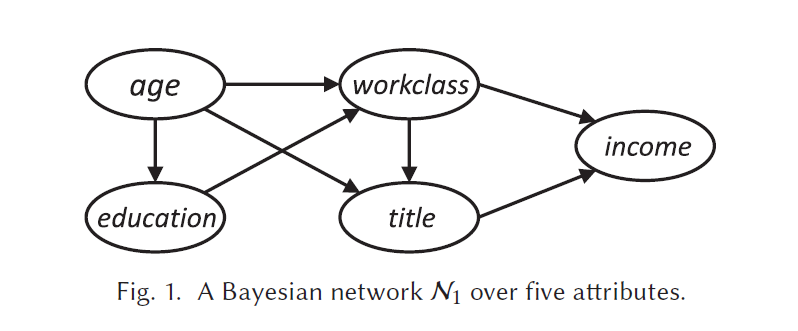
\includegraphics[scale=.35]{../graphs/figure_1.PNG}
\end{figure}
\begin{itemize}
    \item In Fig. 1, $\mathcal{N} = 2$, but not known in reality
\end{itemize}
}

% \frame{\frametitle{Efficiency - Duration (in seconds)}
% \vskip -2mm
% \begin{table}[!h]
%     \centering
%     \rowcolors{1}{white}{lightgray}
%     \resizebox{\textwidth}{!}{% latex table generated in R 4.4.0 by xtable 1.8-4 package
% Fri Jul 19 16:14:31 2024
\begin{tabular}{llrrrr}
  \toprule
version & description & ctgan & datasynthesizer & synthpop (csv) & synthpop (package) \\ 
  \midrule
v00 & Raw (SD2011) & 331.01 & 245.37 & 2132.12 & 5474.39 \\ 
  v01 & Without eduspec or wkabdur & 290.30 & 264.43 & 10.99 & 8.45 \\ 
  v02 & Without wkabdur & 337.07 & 351.76 & 13.96 & 11.02 \\ 
  v03 & Without eduspec & 306.46 & 351.24 & 11.39 & 8.92 \\ 
  v04 & Last variables: eduspec-wkabdur & 374.57 & 344.02 & 14.23 & 287.85 \\ 
  v05 & Last variables: wkabdur-eduspec & 419.60 & 339.92 & 14.60 & 3657.55 \\ 
  v06 & as.numeric(wkabdur) and last variable: eduspec & 356.02 & 347.36 & 14.12 & 11.05 \\ 
  v07\_1\_20 & + 1 factor variable (20 values) & 339.05 & 264.96 & 42.23 &  \\ 
  v07\_1\_25 & + 1 factor variable (25 values) & 400.28 & 326.84 & 137.47 &  \\ 
  v07\_1\_30 & + 1 factor variable (30 values) & 339.73 & 269.72 & 363.18 &  \\ 
  v07\_2\_20 & + 2 factor variable (20 values) & 369.74 & 339.45 & 74.96 &  \\ 
  v07\_2\_25 & + 2 factor variable (25 values) & 364.56 & 361.81 & 631.43 &  \\ 
  v07\_2\_30 & + 2 factor variable (30 values) & 373.25 & 346.15 & 1222.54 &  \\ 
  v07\_3\_20 & + 3 factor variable (20 values) & 393.99 & 369.58 & 122.77 &  \\ 
  v07\_3\_25 & + 3 factor variable (25 values) & 401.03 & 383.40 & 881.53 &  \\ 
  v07\_3\_30 & + 3 factor variable (30 values) & 394.44 & 424.64 & 3654.59 &  \\ 
   \bottomrule
\end{tabular}
}
%     \label{table_sd2011_duration.tex}
% \end{table}
% }


\frame{\frametitle{SD2011 - pMSE}
\vskip -2mm
\begin{figure}
    \resizebox{.75\textwidth}{!}{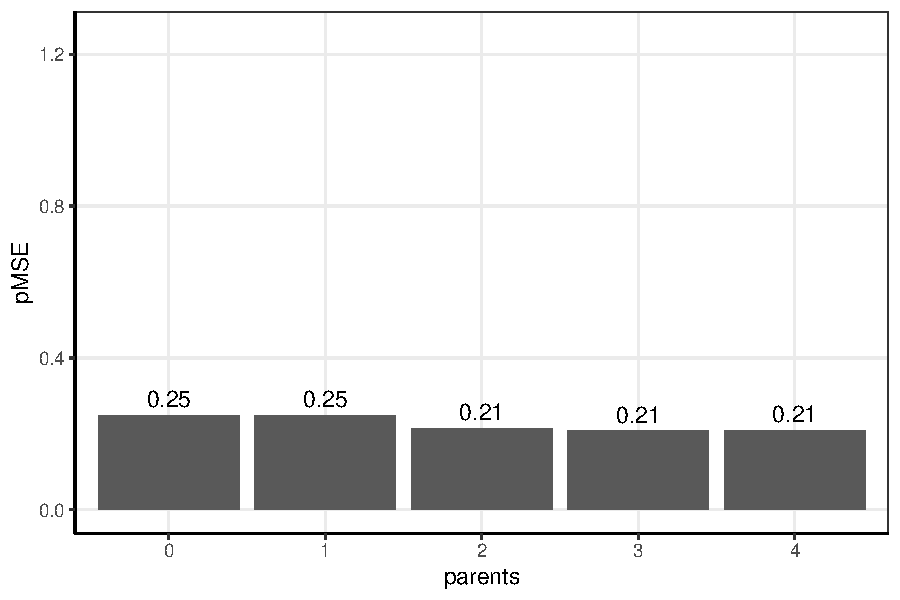
\includegraphics{../graphs/datasynthesizer/datasynthesizer_fidelity_optimize_dataset_parents.pdf}}
    \label{fig:datasynthesizer_fidelity_optimize_dataset_parents}
\end{figure}
}

\frame{\frametitle{DataSynthesizer - SD2011(a)}
\vskip -2mm
\begin{figure}
    \resizebox{.75\textwidth}{!}{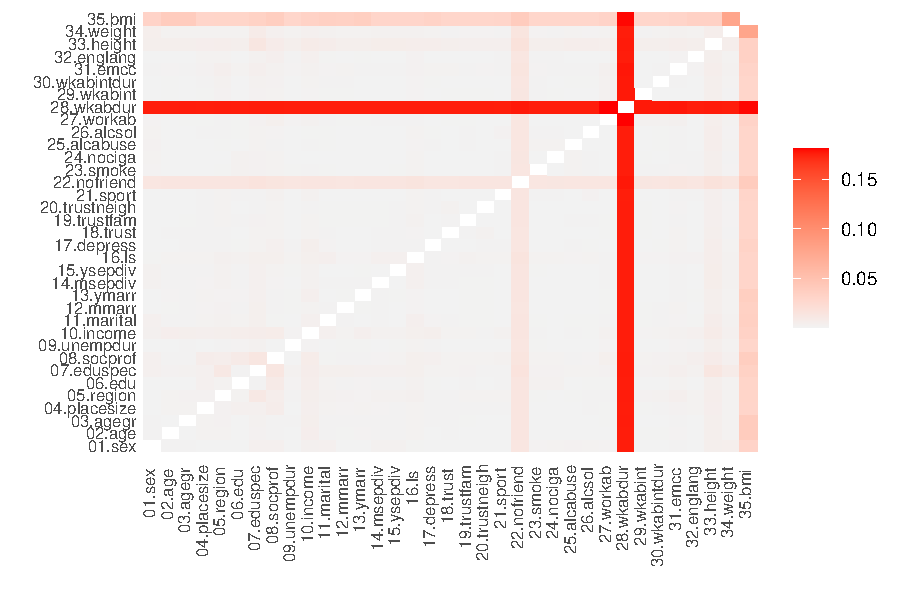
\includegraphics{../graphs/datasynthesizer/datasynthesizer_fidelity_twoway_sd2011_presentation.pdf}}
    \label{fig:ds_fidelity_two_way_subfig-a}
\end{figure}
}

\frame{\frametitle{variable: wkabdur (Work abroad duration)}
\vskip -2mm
\begin{figure}
    \resizebox{.75\textwidth}{!}{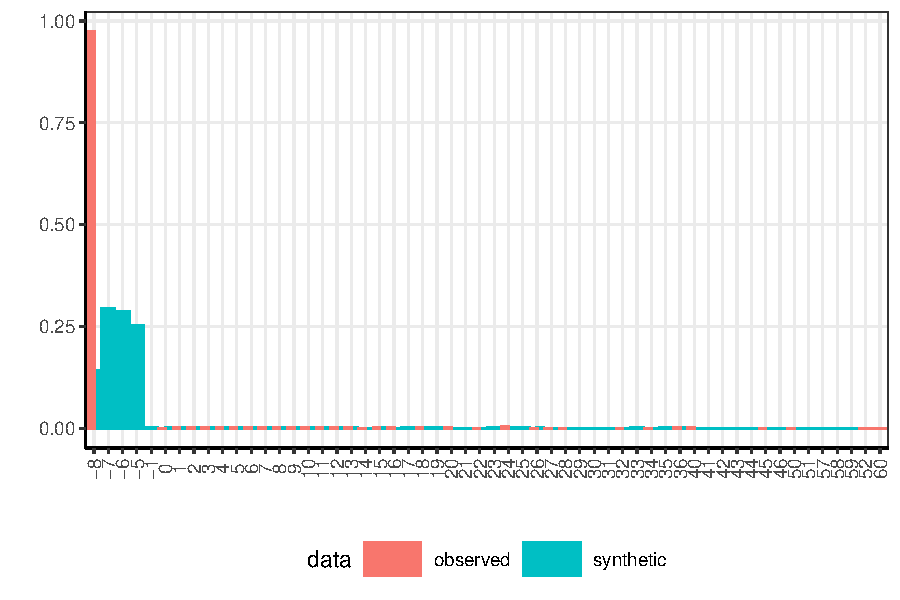
\includegraphics{../graphs/datasynthesizer/datasynthesizer_wkabdur.pdf}}
    \label{fig:ds_variable_wkabdur}
\end{figure}
}

\frame{\frametitle{DataSynthesizer - SD2011(b)}
\vskip -2mm
\begin{figure}
    \resizebox{.75\textwidth}{!}{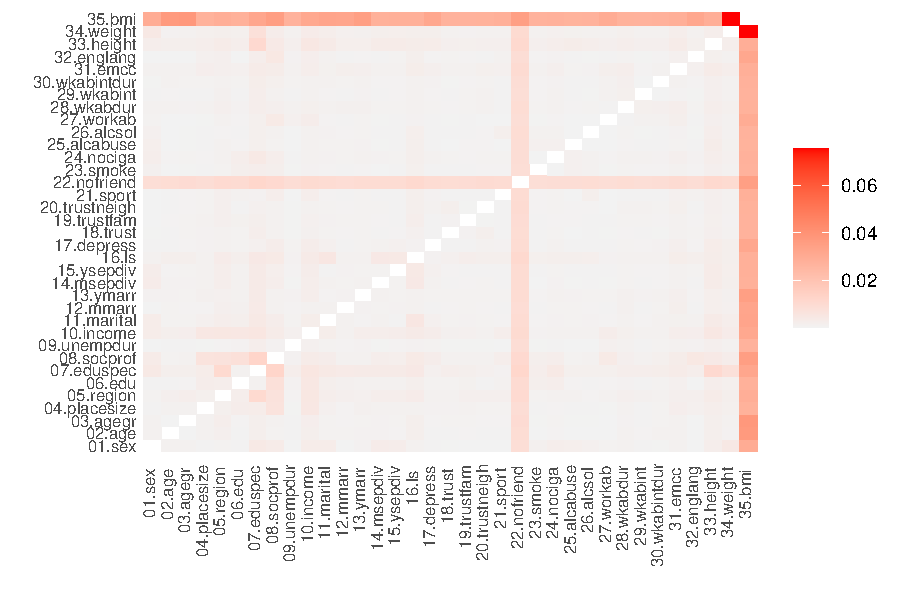
\includegraphics{../graphs/datasynthesizer/datasynthesizer_fidelity_twoway_sd2011_clean_presentation.pdf}}
    \label{fig:ds_fidelity_two_way_subfig-b}
\end{figure}
}

\frame{\frametitle{variable: bmi}
\vskip -2mm
\begin{figure}
    \caption{BMI $<$ 20 is underweight/malnourished}
\vskip -2mm
    \resizebox{.7\textwidth}{!}{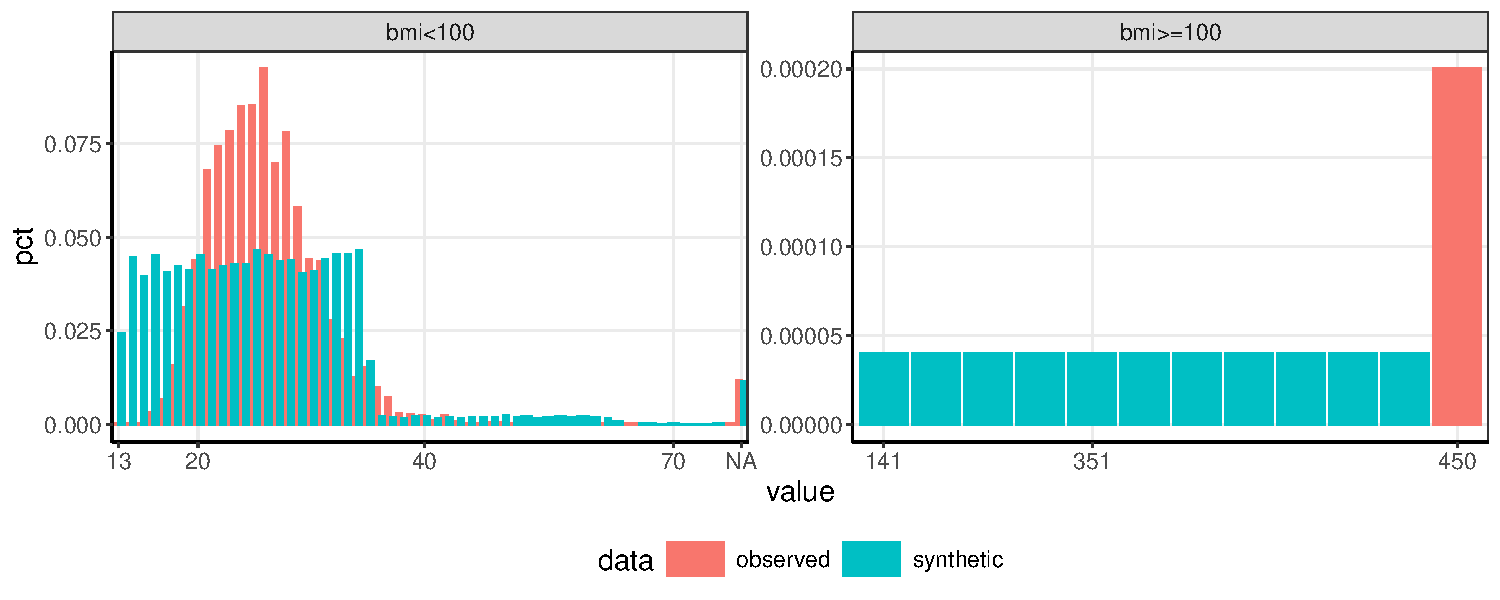
\includegraphics{../graphs/datasynthesizer/datasynthesizer_bmi.pdf}}
    \label{fig:ds_variable_bmi}
\end{figure}
}

\frame{\frametitle{DataSynthesizer - SD2011(c)}
\vskip -2mm
\begin{figure}
    \resizebox{.75\textwidth}{!}{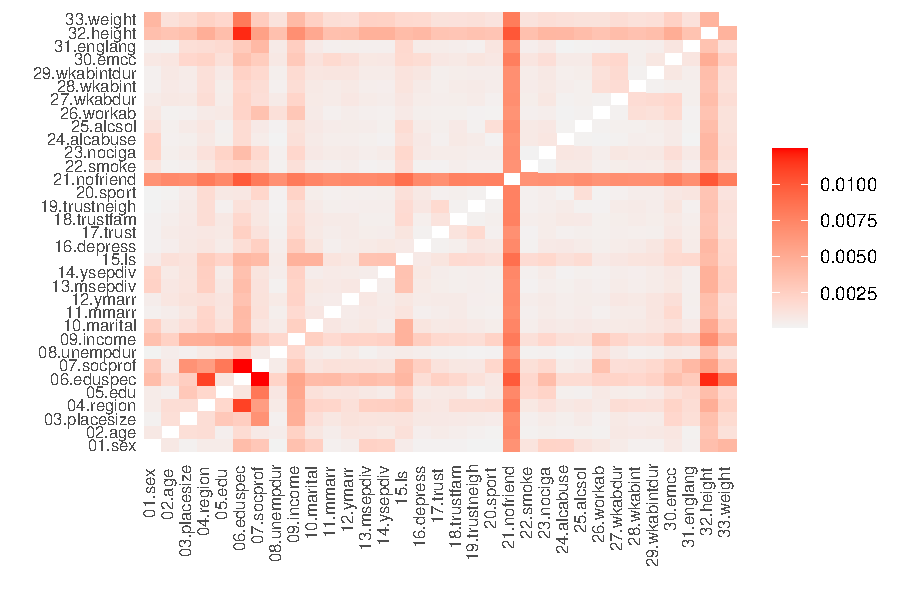
\includegraphics{../graphs/datasynthesizer/datasynthesizer_fidelity_twoway_sd2011_clean_small_presentation.pdf}}
    \label{fig:ds_fidelity_two_way_subfig-c}
\end{figure}
}

\frame{\frametitle{variable: nofriend}
\vskip -2mm
\begin{figure}
    \caption{Doesn't capture rounding/discontinuity}
\vskip -2mm
    \resizebox{.7\textwidth}{!}{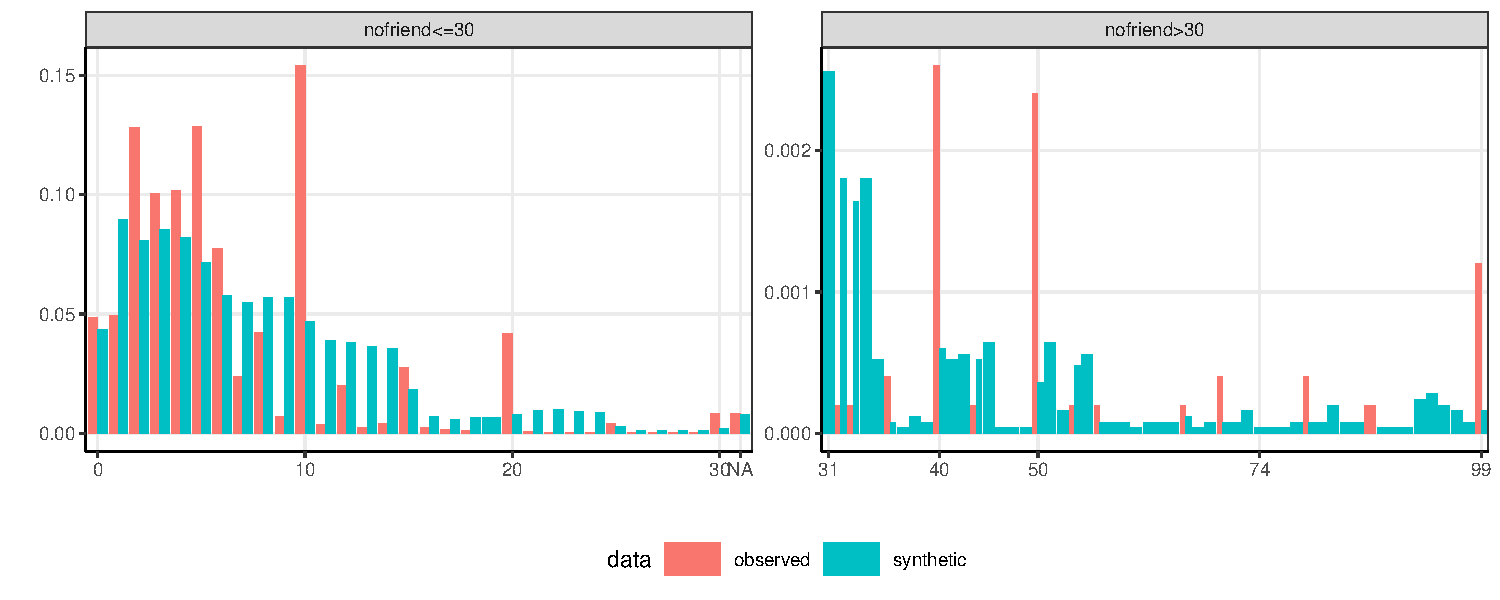
\includegraphics{../graphs/datasynthesizer/datasynthesizer_nofriend.pdf}}
    \label{fig:ds_variable_nofriend}
\end{figure}
}

\frame{\frametitle{SD2011 - pMSE}
\vskip -2mm
\begin{figure}
    \resizebox{.75\textwidth}{!}{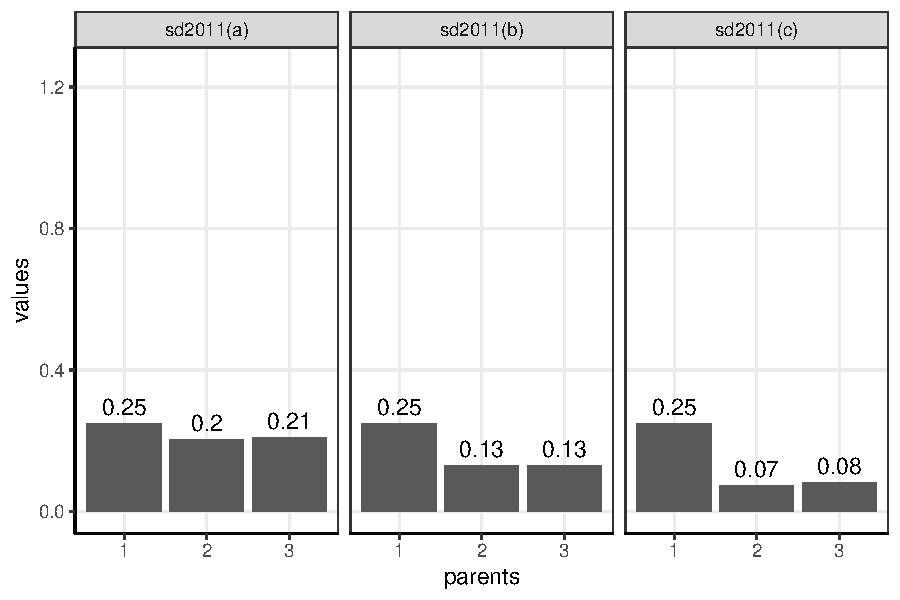
\includegraphics{../graphs/datasynthesizer/datasynthesizer_fidelity_optimize_dataset_parents_compare.pdf}}
    \label{fig:datasynthesizer_fidelity_optimize_dataset_parents_compare}
\end{figure}
}

\frame{\frametitle{Datasynthesizer: selected variables}
\begin{figure}
    \caption{No missings if parents $<$ 2}
    \resizebox{\textwidth}{!}{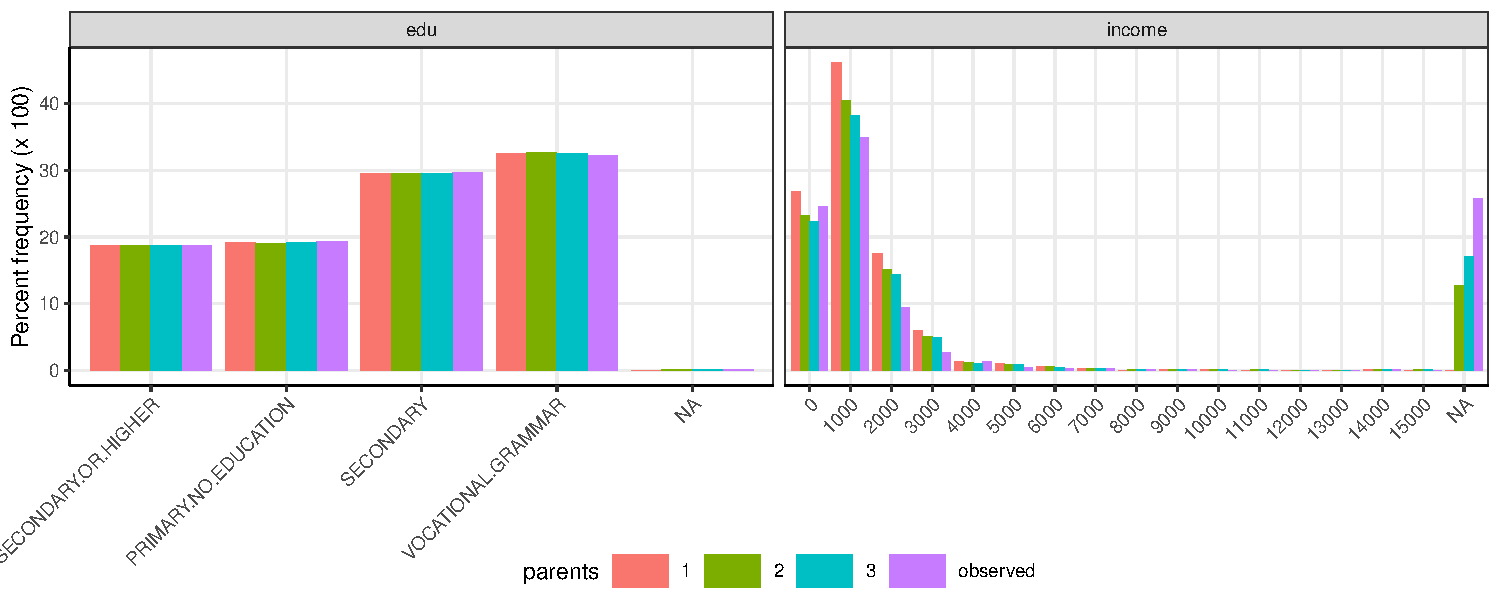
\includegraphics{../graphs/datasynthesizer/datasynthesizer_frequency_optimize_variables_parents.pdf}}
    \label{subfig:tuning_ds_variables_within_synthetic}
\end{figure}
}


\subsection{CTGAN}\label{sec:sdg_ctgan}
\frame[c]{\frametitle{}
\centering
Section \ref{sec:sdg}\ref{sec:sdg_ctgan}: Know your generator (CTGAN)
}

\frame{\frametitle{Tuning CTGAN}
\begin{itemize}
    \item Batch size (constant steps)
    \item Epochs (constant batch size)
    \item Dimensions (2 hyperparameters)
    \begin{itemize}
        \item embedding\_dim (int): Size of the random sample passed to the Generator. Defaults to 128.
        \item dimensionality - 2 hyperparameters, but same value for each
        \begin{itemize}
            \item discriminator\_dim (tuple or list of ints): Size of the output samples for each one of the Discriminator Layers. A Linear Layer will be created for each one of the values provided. Defaults to (256, 256).
            \item generator\_dim (tuple or list of ints): Size of the output samples for each one of the Residuals. A Resiudal Layer will be created for each one of the values provided. Defaults to (256, 256).  
        \end{itemize}
    \end{itemize}
\end{itemize}
}

\frame{\frametitle{Batch size, epochs, and steps}
\begin{table}[!h]
    \rowcolors{1}{white}{lightgray}
    \caption{}
    \centering
    \begin{tabular}{cllll}
    \toprule
    N & Batch size & Steps per Epoch & Epochs & Actual Steps \\
    \midrule
    5.000 & 100 & 50 & 60 & 3,000 \\
    5.000 & 250 & 20 & 150 & 3,000 \\
    5.000 & 500 & 10 & 300 & 3,000 \\
    5.000 & 1.000 & 5 & 600 & 3,000 \\ \hline
    5.000 & 500 & 10 & 100 & 1,000 \\
    5.000 & 500 & 10 & 300 & 3,000 \\
    5.000 & 500 & 10 & 600 & 6,000 \\
    5.000 & 500 & 10 & 900 & 9,000 \\
    \bottomrule
    \end{tabular}
\end{table}
}

% \section{Results}\label{sec:results}
\frame{\frametitle{CTGAN: Effect of batch size (constant steps)}
\begin{figure}
    \resizebox{.75\textwidth}{!}{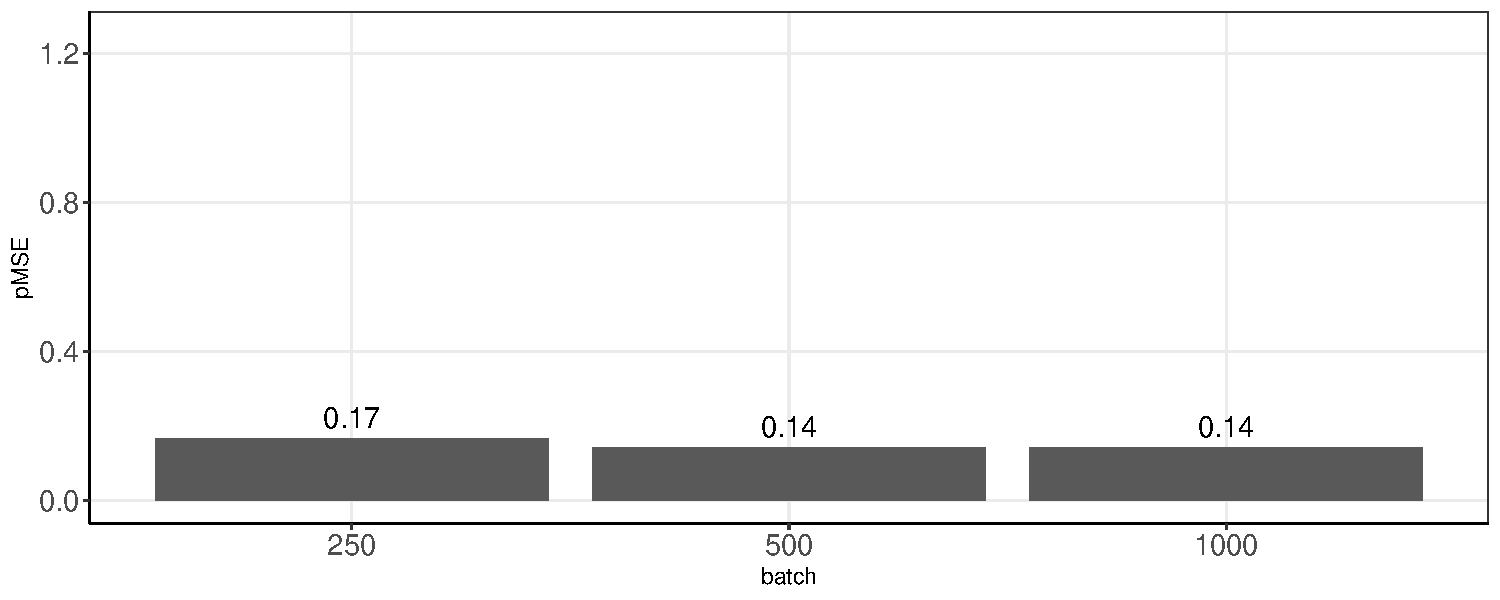
\includegraphics{../../ctgan/graphs/ctgan/ctgan_fidelity_optimize_batch_size.pdf}}
    \label{ctgan_fidelity_optimize_batch_size}
\end{figure}
}

\frame{\frametitle{CTGAN: Effect of epochs (constant batch size)}
\begin{figure}
    \resizebox{.75\textwidth}{!}{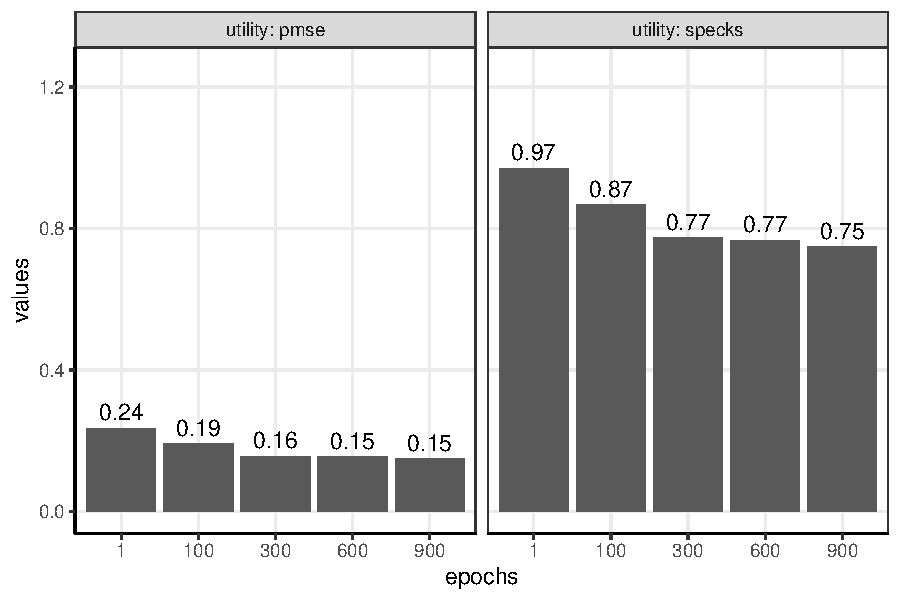
\includegraphics{../../ctgan/graphs/ctgan/ctgan_fidelity_optimize_epochs.pdf}}
    \label{ctgan_fidelity_optimize_epochs}
\end{figure}
}

\frame{\frametitle{CTGAN: Effect of dimensions}
\begin{figure}
    \resizebox{.7\textwidth}{!}{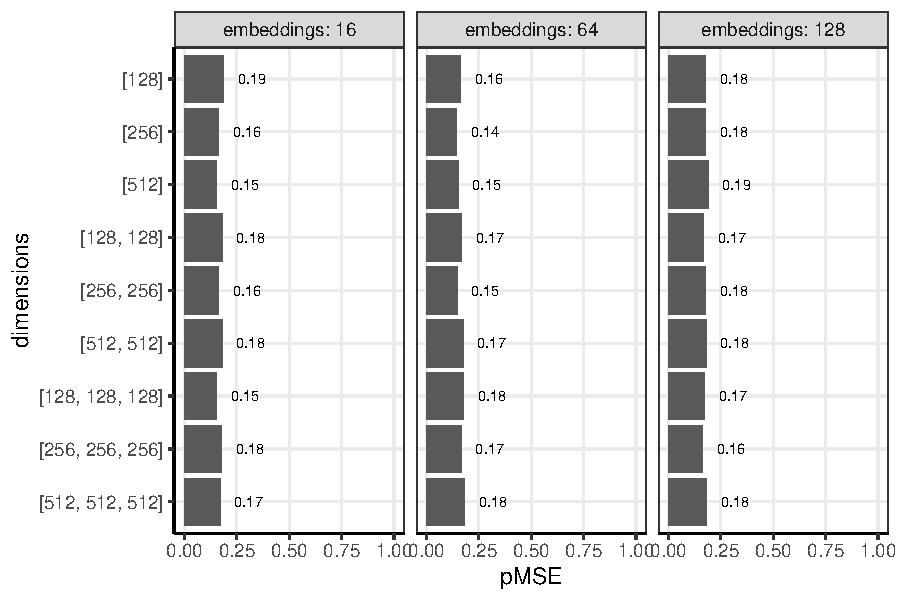
\includegraphics{../../ctgan/graphs/ctgan/ctgan_fidelity_optimize_dimensions.pdf}}
    \label{ctgan_fidelity_optimize_dimensions}
\end{figure}
}

\subsection{Synthpop}\label{sec:sdg_synthpop}
\frame[c]{\frametitle{}
\centering
Section \ref{sec:sdg}\ref{sec:sdg_ctgan}: Know your generator (Synthpop)
}

\section{Conclusion}\label{sec:conclusion}
\frame[c]{\frametitle{}
\centering
Section \ref{sec:conclusion}: Conclusion
}


\end{spacing}
\end{document}

